
%%%%%%%%%%%%%%%%%%%% ahm_icsc2026.tex %%%%%%%%%%%%%%%%%%%%
% AHM: Embedding Live Machine Learning in Csound
% Submission to ICSC 2026
%%%%%%%%%%%%%%%%%%%%%%%%%%%%%%%%%%%%%%%%%%%%%%%%%%%%%%%%%%

\documentclass[runningheads,a4paper]{llncs}

\usepackage[T1]{fontenc}
\usepackage{amssymb}
\setcounter{tocdepth}{3}
\usepackage{graphicx}
\graphicspath{{.}{../Figure/}}
\usepackage{hyperref}
\usepackage[top=1.0in,bottom=1.0in,left=0.95in,right=0.95in]{geometry}
\hypersetup{hidelinks}

\newcommand{\keywords}[1]{\par\addvspace\baselineskip
\noindent\keywordname\enspace\ignorespaces#1}

\pagestyle{headings}

\begin{document}

\mainmatter

\title{Embedding Live Machine Learning in Csound:\texorpdfstring{\\}{ }%
Emotion-Driven Harmony via an ONNX-Runtime Opcode}

\titlerunning{Live ML Inference in Csound for Emotion-Driven Harmony}

% TO GUARANTEE THE DOUBLE BLIND REVIEW PROCESS, PLEASE
% KEEP THESE GENERIC AUTHOR NAMES AND INSTITUTIONS
\author{Anonymous Author(s)}
\authorrunning{Anonymous Author(s)}
\institute{Anonymous Institution \\
\email{anonymous@example.com}}

\maketitle

\begin{abstract}
Harmonic generation in Csound typically requires explicit chord specification
in the score or coordination with an external process. We present the
\emph{Affective Harmony Machine} (AHM), a system that embeds an ONNX-format
machine-learning model as a native Csound opcode, demonstrated through
affect-driven chord progression generation. The system is backed by
an annotated dataset of 108 jazz and pop chord progressions labeled with six
emotion classes and seven scale/mode categories. A Random Forest classifier trained on
this dataset is exported to the ONNX interchange format. The authors created
\texttt{emoChord}, a Csound opcode that accepts an emotion string, performs live
ML inference at i-rate via the ONNX Runtime C~API, and schedules harmonically
appropriate chord events into a synthesis instrument. No Python interpreter or
external process is required at runtime; the current release targets macOS
(arm64 natively, x86\_64 via Rosetta). The implementation demonstrates
a general pattern for embedding ONNX-compatible classifiers in Csound as a
native plugin with no Python runtime requirement.
\keywords{Csound opcode, ONNX Runtime, machine learning, harmony generation,
emotion, chord progression, affective computing}
\end{abstract}


\section{Introduction}

Csound~\cite{lazzarini2016} has a long tradition of algorithmic composition,
from Lorrain's stochastic cannons~\cite{lorrain1980} to contemporary generative
harmony and algorithmic interactive systems. Yet in most of these systems, harmony
remains the composer's explicit responsibility: chords are either written into
the score by hand or drawn from probability tables constructed in advance.
Shi and Boulanger's CStore~\cite{shi2026} demonstrated AI-driven orchestra
code from natural language, though as an external process, sharpening
the question: how far can machine intelligence be embedded \emph{within}
Csound itself?

We answer concretely: any ONNX-compatible classifier following the same
input/output tensor contract can be embedded as a native Csound i-rate opcode
via the ONNX Runtime C~API with no external-process dependency.
As a demonstration, the \emph{Affective Harmony Machine} (AHM) targets
affect-driven harmony, where emotional states map to musical parameters such as
mode and perceived affect~\cite{hevner1935}: a composer writes \texttt{i1~0~4~"joyful"}
to receive chord events: MIDI-pitched notes inserted at i-rate via
Csound's score API (Section~\ref{sec:pipeline}) into any synthesis instrument.


\section{Dataset}

The system is trained on two curated harmony corpora. The jazz dataset covers
functional harmony, including secondary dominants, tritone substitutions, and
deceptive resolutions, across 25 unique progressions, each realized in four jazz
voicing styles (Four-Way Close, Drop~2, Drop~3, Drop~2+4); the four variants
share the same progression class label; voicing style is an auxiliary label
for a co-trained classifier, not part of the 108-class target. All progressions
and voicing assignments were hand-coded by the authors.\footnote{\url{https://anonymous.4open.science/r/AHM-Dataset-8F24/README.md}} The pop dataset covers
diatonic, modal, and borrowed-chord idioms across 83 unique progressions.
Table~\ref{tab:dataset} summarizes the combined dataset.

\begin{table}[t]
\caption{Dataset summary after preprocessing.}
\label{tab:dataset}
\centering
\begin{tabular}{lccc}
\hline
Source & Progressions & Rows & Coverage \\
\hline
Jazz      & 25 & 1{,}200 & 12 keys $\times$ 4 voicings \\
Pop       & 83 &   996   & 12 keys \\
\textbf{Combined} & \textbf{108} & \textbf{2{,}196} & $-$ \\
\hline
\end{tabular}
\end{table}

Each row is annotated along three orthogonal dimensions: \textbf{Emotion}
(6~classes: Joyful, Vital, Epic, Uneasiness, Depressive, Despair)\footnote{Labels
were defined by the authors and intentionally mix grammatical forms (adjective,
noun, etc.) as classification shorthand; a principled affect taxonomy is a
planned direction (Section~\ref{sec:future}).},
\textbf{Scale/Mode} (7~classes: Ionian, Aeolian, Dorian, Phrygian, Lydian,
Mixolydian, Harmonic minor), and \textbf{Key} (Key is represented as one of 12 pitch centers rather than as 24 major/minor keys, since mode is encoded separately by the Scale/Mode label).
Progressions are encoded in Roman numeral notation (\textit{e.g.,}~\texttt{I-V-vi-IV}),
making the representation key-invariant: the model learns harmonic character,
not absolute pitch. Pop progressions were expanded to all 12~keys via automated
transposition using key-aware enharmonic spelling tables, ensuring balanced class
coverage across all keys. Emotion and scale annotations follow established modal conventions. The six
emotion classes were consolidated from thirteen original categories for
broader affective coverage.


\section{Machine Learning Pipeline}

\subsection{Feature Design}

The classification task is: \emph{given (emotion, scale), predict the most
probable chord progression type}, a 2-input, 108-class problem. Key is
intentionally excluded from the feature vector because transposition does not
alter harmonic character, and including it would fragment the training data into
24 identical shards. Both inputs are label-encoded to integer indices;
the feature matrix is shape $[N \times 2]$ (float32), and the target indexes
one of 108 progression classes. The dataset spans 23 of the 42 possible
\texttt{(emotion, scale)} combinations; the model learns a distinct probability
distribution over the 108 classes for each observed pair, enabling
temperature-weighted sampling rather than a fixed argmax lookup.

\subsection{Random Forest with Optuna Tuning}

A Random Forest Classifier~\cite{sklearn2011} is chosen because its
\texttt{predict\_proba()} output provides a per-class probability vector over
all 108 progression types, directly usable as a stochastic sampling distribution
at runtime; the downstream temperature scaling and weighted sampling
(Section~\ref{sec:temp}) act on this vector to enable probabilistic affective
selection.

Hyperparameters are optimized with Optuna~\cite{optuna2019} (50~trials, 5-fold CV;
the training script co-tunes a jazz voicing classifier, but only the progression
model is exported). Training follows a two-stage procedure:
hyperparameter search on an 80/20 stratified split, then retraining on the
complete 2{,}196-row dataset. Retraining is critical: stratification by emotion
(6~classes) rather than the 108-class target means rare progressions absent
from the 80\% fold would break index mappings at runtime.

\subsection{ONNX Export}

The trained classifier is exported with \texttt{skl2onnx}~\cite{skl2onnx}
using \texttt{zipmap=False}, which produces a plain float32 tensor
\texttt{"probabilities"}~$[N, 108]$ enabling direct array access from C, and
\texttt{target\_opset=18} to match the bundled ONNX Runtime version. The
resulting \texttt{gen\_model.onnx} encodes the full Random Forest decision
structure with no Python dependency. A companion vocabulary table
\texttt{gen\_data.tsv} (108 progressions $\times$ 12 pitch classes = 1{,}296 rows)
maps each progression ID to one canonical chord-name string per pitch class;
jazz voicing variants share the same progression class and are not represented
as separate runtime entries, with major/minor spellings handled according to scale context.


\section{Embedding ML in a Csound Opcode}

\subsection{Overview}

The key contribution of AHM is that ML inference runs natively inside the Csound
process. The authors built the plugin as a \texttt{.dylib} that links directly
against the ONNX Runtime C library~\cite{onnxruntime};
\texttt{emoChord\_init SModelPath, SDataPath} loads the ONNX model and
vocabulary table once at i-rate, storing all shared state in static C globals available to every subsequent
\texttt{emoChord} call (not thread-safe across concurrent Csound instances). Figure~\ref{fig:arch}
shows the two-phase architecture.

\begin{figure}[t]
\centering
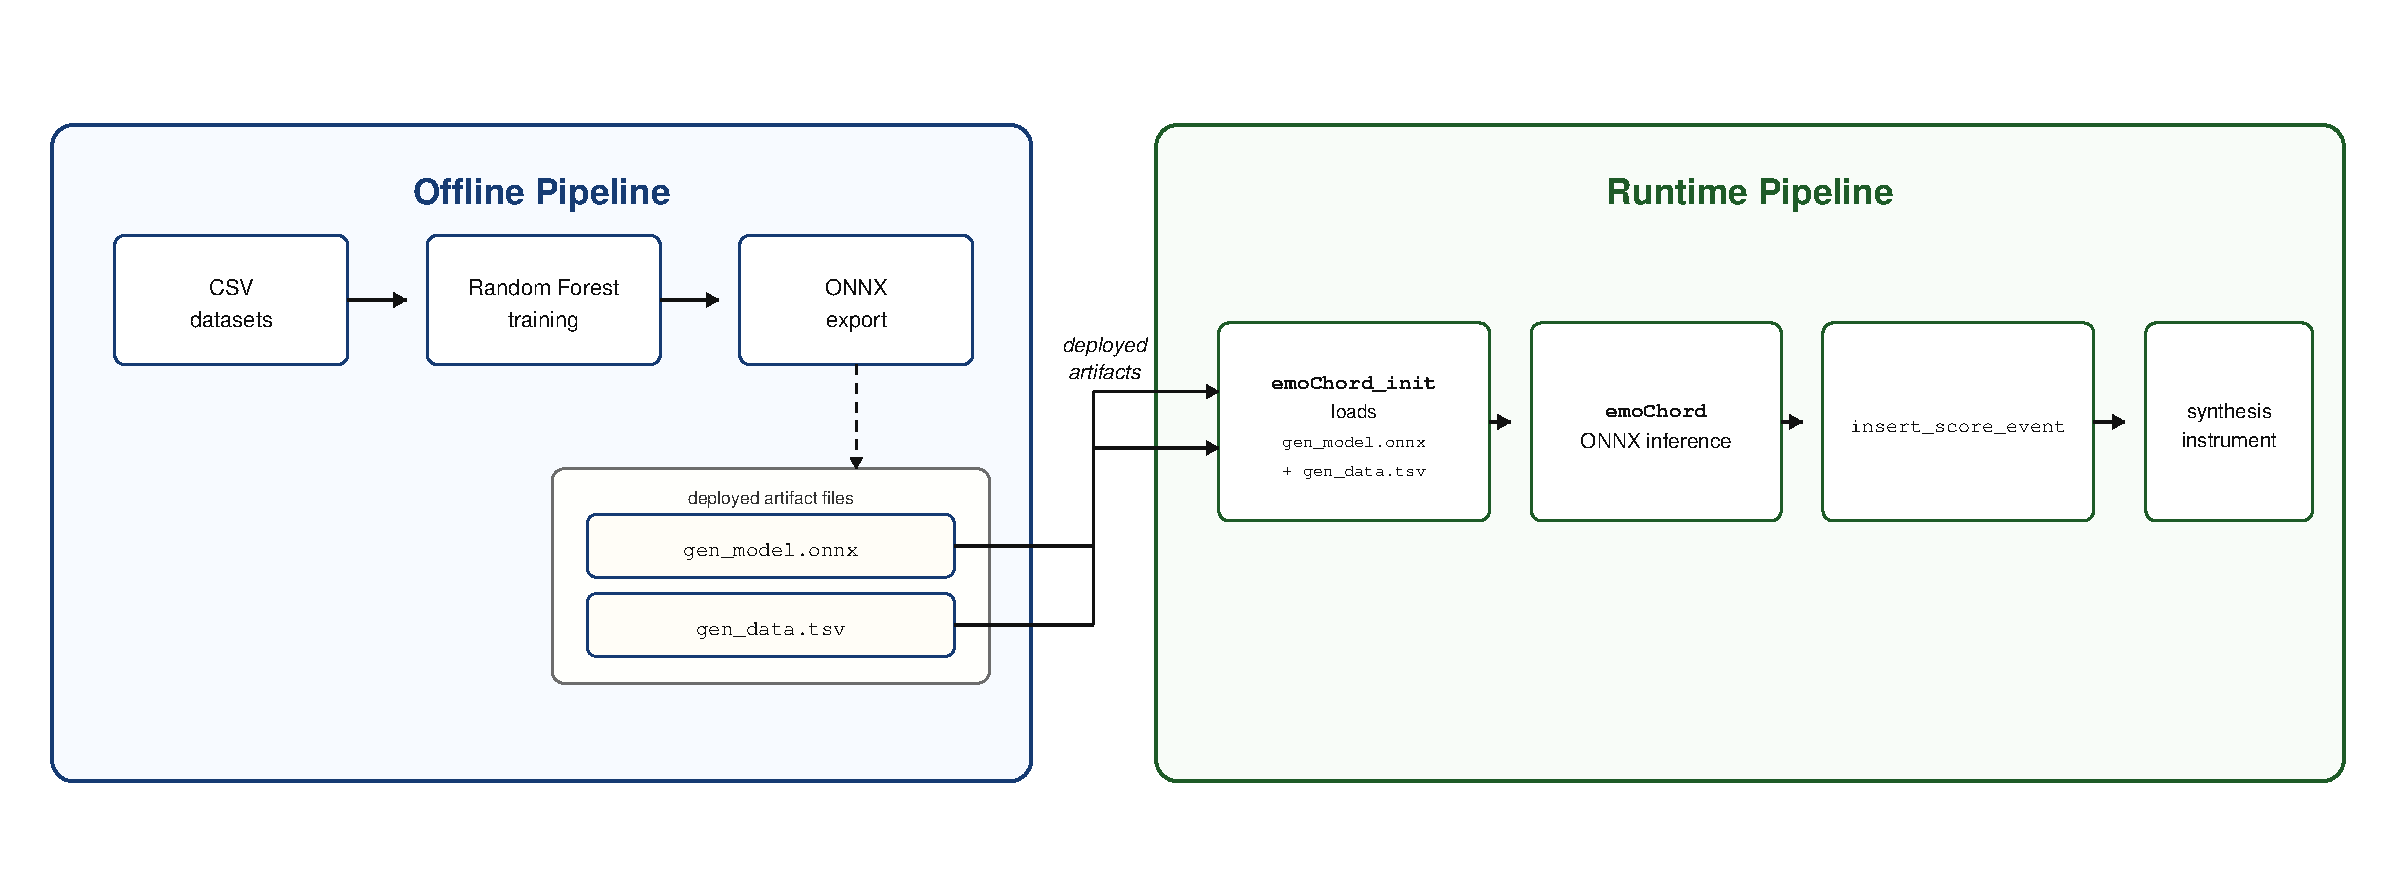
\includegraphics[width=0.95\linewidth]{architecture_pipeline.pdf}
\caption{AHM two-phase architecture. Offline (left): training and ONNX export
of \texttt{gen\_model.onnx} and \texttt{gen\_data.tsv}. Runtime (right): native
Csound inference and chord event scheduling via \texttt{emoChord}.}
\label{fig:arch}
\end{figure}

No external process is needed at runtime. Inference runs at i-rate; on Apple
Silicon (arm64), median single-sample inference is 14~$\mu$s, far below typical score-event
scheduling timescales, and model load is 52~ms.

\subsection{Live Inference Pipeline in \texttt{emoChord}}
\label{sec:pipeline}

{\small\texttt{emoChord SEmotion, iInstr, iStart, iDur, iAmp [, iTemp, iOctave]}}
executes the following seven-step pipeline entirely inside the Csound process:

\begin{enumerate}\setlength{\itemsep}{1pt}\setlength{\parskip}{0pt}
\item \textbf{Resolve emotion}: scan \texttt{DataEntry[]} for rows matching
  \texttt{SEmotion} (case-insensitive) to obtain \texttt{emotion\_id}.
\item \textbf{Sample scale}: collect all \texttt{scale\_id} values for that
  emotion, weighted by dataset frequency; draw one by temperature-weighted
  inverse-CDF.
\item \textbf{ONNX inference}: call \texttt{OrtApi->Run()} with input
  $[1,2] = \{\mathit{emotion\_id},\,\mathit{scale\_id}\}$, retrieving
  $\mathbf{p} \in \mathbb{R}^{108}$.
\item \textbf{Filter}: mask $\mathbf{p}$ to \texttt{prog\_id} values present
  for the sampled pair; guaranteed non-empty by construction, since Step~2
  draws only from \texttt{scale\_id} values observed for the given emotion.
\item \textbf{Temperature scaling}: apply $p'_i = p_i^{1/T}$ and renormalize
  over the filtered candidates.
\item \textbf{Sample progression}: draw one \texttt{prog\_id} by weighted
  inverse-CDF.
\item \textbf{Schedule chords}: look up the \texttt{chord\_name} string
  (\textit{e.g.,}~\texttt{Cm7-F7-Bbmaj7}), parse tokens into MIDI note
  numbers, and call \texttt{insert\_score\_event()} on instrument
  \texttt{iInstr}.
\end{enumerate}

\subsection{Temperature as Compositional Control}
\label{sec:temp}

The \texttt{iTemp} parameter (default~1.0) translates the ML temperature concept
into a direct musical control. At low $T$ sampling concentrates on the highest-probability progression; at
$T = 1$ it follows the model's trained
distribution; at $T > 1$ the distribution flattens toward uniform, increasing
harmonic variety. A composer can place two adjacent score events with the same
emotion string but different temperatures: one to anchor a phrase and one to
introduce a surprise chord, without touching the model or any other instrument
parameter.

\subsection{Usage Example}

Listing~1 shows a minimal \texttt{.csd}. Instrument~1 reads an emotion string
via \texttt{strget} and passes it to \texttt{emoChord}, which schedules events
into any target instrument. Figure~\ref{fig:output} shows the console output for the three events in Listing~1.

\medskip
\noindent{\it Listing 1: Minimal \texttt{emoChord} usage.}
{\small\begin{verbatim}
<CsInstruments>
emoChord_init "/path/to/gen_model.onnx", \
              "/path/to/gen_data.tsv"
instr 1 
  Sem strget p4 ; p4=emotion string
  emoChord Sem, 2, p2, p3, 0.7
endin
</CsInstruments>
<CsScore>
i1  0  4  "joyful"
i1  6  4  "depressive"
i1 12  4  "uneasiness"
e
</CsScore>
\end{verbatim}}

Passing the emotion as a score p-field follows the standard Csound
idiom~\cite{boulanger2011,boulanger2000}. At each event, \texttt{emoChord} prints the
selected progression (\textit{e.g.,}~\texttt{[emoChord] "joyful" -> Ionian
-> C-G-Am-F}), making ML choices transparent during composition.

\begin{figure}[h]
\centering
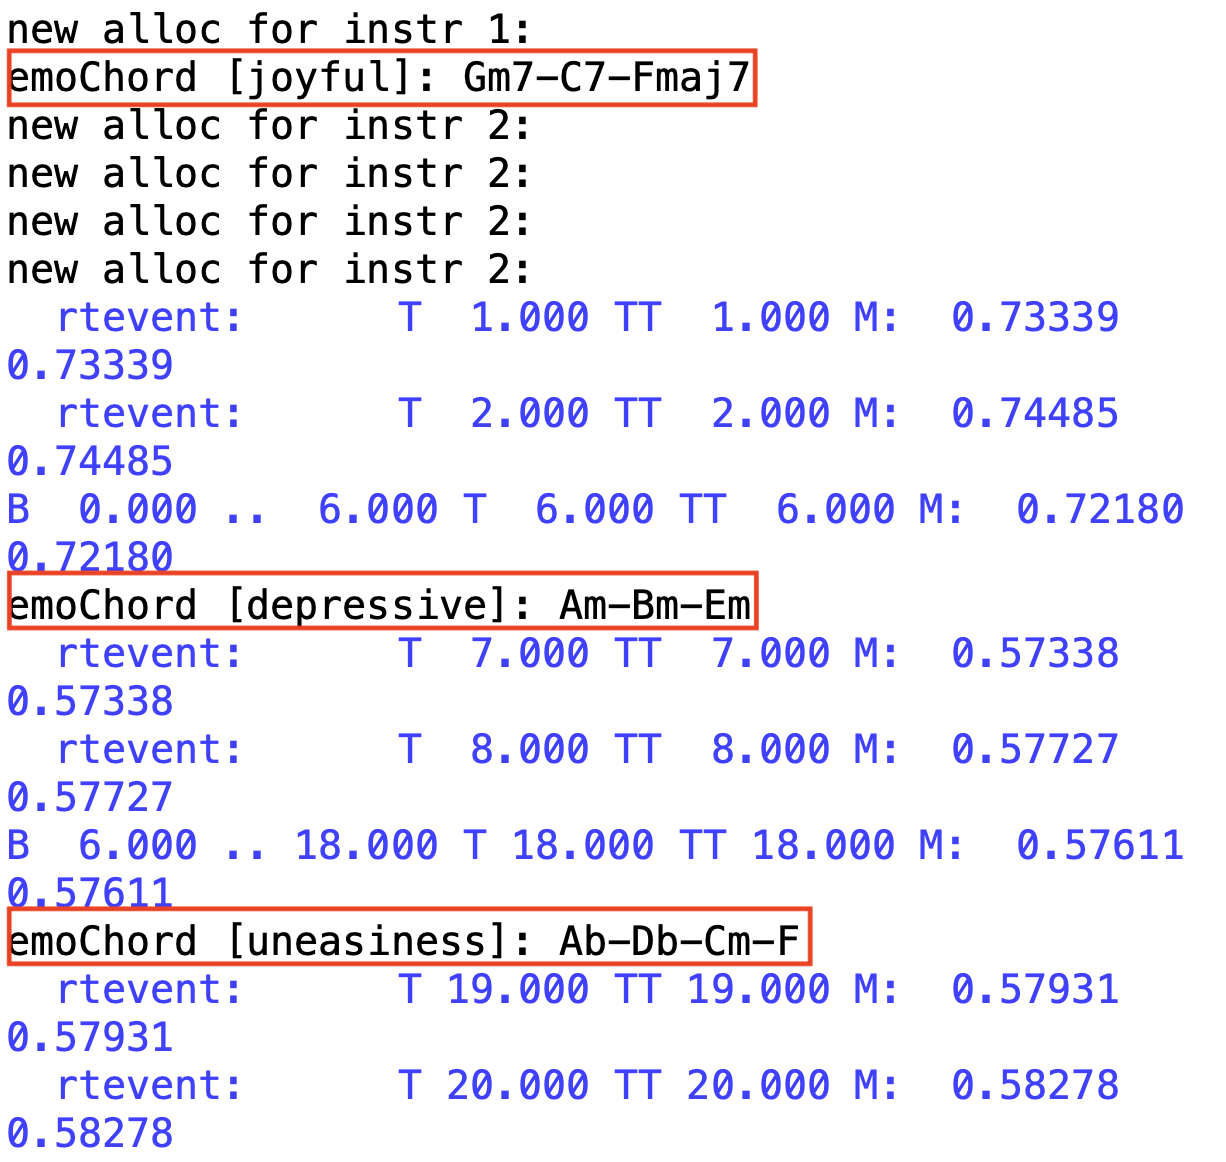
\includegraphics[height=5.2cm]{Output}
\caption{\texttt{emoChord} console output for three score events.}
\label{fig:output}
\end{figure}


\section{Results and Conclusion}

After Optuna tuning (50~trials, 5-fold CV), the model achieves held-out top-1
accuracy of 24.8\% and top-3 of 49.1\%, against a uniform random baseline of
0.9\% (1/108) and a majority-class-per-pair baseline of 24.8\%. The latter
confirms the model has learned the dominant harmonic preference per
\texttt{(emotion, scale)} cell; the accuracy ceiling is a design property,
since feature vectors within a cell are identical and bounded by the
dominant-class proportion. The model's purpose is to package the learned
distribution as an ONNX tensor: at $T\to 0$ it reduces to a majority lookup,
while temperature sampling exposes the full distribution to the composer.

The dataset built for this work, combining 2{,}196 rows of jazz and pop
progressions under a unified six-class affect taxonomy, is itself a contribution
we hope will prove useful to others; we believe this combination to be a first,
though the area is broad. Beyond the dataset, the pattern this work establishes
is that domain-specific ML is a practical candidate for native Csound integration:
a composer writes one emotion word into a score and receives chord events, with
all inference invisible inside the process. Any ONNX classifier with a compatible
tensor contract can replace the current model without touching the plugin.
Anonymized code and data are available at \url{https://anonymous.4open.science/r/AHM-Dataset-8F24/README.md}


\section{Future Directions}
\label{sec:future}

Planned extensions include a genre input to resolve jazz/pop ambiguity,
longer sequence generation, a free-text prompt interface mapping natural-language
input to the nearest \texttt{(emotion, scale)} pair, a k-rate variant,
an \texttt{iKey} parameter, emotion label standardization, a perceptual
evaluation, and Windows/Linux porting. The authors continue to expand the dataset and refine the model; updated releases will be posted to the project repository as work progresses.


{\small\begin{thebibliography}{10}

\bibitem{shi2026}
Shi, L.C., Boulanger, R.: CStore: A Framework for Generating Editable,
Versionable Csound Orchestra Code -- From Text to Sound and Music. In:
Proceedings of the 2026 IEEE Conference on Artificial Intelligence (CAI),
pp.~237--243. IEEE, Granada (2026)

\bibitem{lorrain1980}
Lorrain, D.: A panoply of stochastic cannons. Computer Music Journal 4(1),
53--81 (1980)

\bibitem{hevner1935}
Hevner, K.: The affective character of the major and minor modes in music.
American Journal of Psychology 47, 103--118 (1935)

\bibitem{sklearn2011}
Pedregosa, F. et al.: Scikit-learn: Machine Learning in Python. Journal of
Machine Learning Research 12, 2825--2830 (2011)

\bibitem{optuna2019}
Akiba, T., Sano, S., Yanase, T., Ohta, T., Koyama, M.: Optuna: A
next-generation hyperparameter optimization framework. In: Proceedings of the
25th ACM SIGKDD International Conference on Knowledge Discovery \& Data Mining,
pp.~2623--2631 (2019)

\bibitem{skl2onnx}
Dupré, X. et al.: sklearn-onnx: Convert scikit-learn models to ONNX.
\url{https://onnx.ai/sklearn-onnx/} (2019--present)

\bibitem{onnxruntime}
ONNX Runtime Developers: ONNX Runtime inference engine.
\url{https://onnxruntime.ai} (2018--present)

\bibitem{lazzarini2016}
Lazzarini, V. et al.: Csound: A Sound and Music Computing System.
Springer, Cham (2016)

\bibitem{boulanger2011}
Boulanger, R., Lazzarini, V. (eds.): The Audio Programming Book.
MIT Press, Cambridge (2010)

\bibitem{boulanger2000}
Boulanger, R. (ed.): The Csound Book: Perspectives in Software Synthesis,
Sound Design, Signal Processing, and Programming.
MIT Press, Cambridge (2000)

\end{thebibliography}}

\end{document}
